
\documentclass{kththesis}

\usepackage{graphicx}
\usepackage{todonotes}
\usepackage{blindtext} % This is just to get some nonsense text in this template, can be safely removed
\usepackage{hyperref}
\usepackage{subcaption}
\usepackage{array}
\usepackage{enumitem}

\usepackage{xcolor}

\usepackage{csquotes} % Recommended by biblatex
\usepackage[style=numeric,sorting=none,backend=biber]{biblatex}
\addbibresource{references.bib} % The file containing our references, in BibTeX format
\title{Comparison of Progressive Web Apps and Mobile Applications on Android}
\alttitle{Jämförelse av progressiva webbappar och mobilapplikationer på Android}
\author{Camille Fournier}
\email{camillef@kth.se}
\supervisor{Javier Cabrera-Arteaga}
\examiner{Benoit Baudry}
\hostcompany{Odiwi} % Remove this line if the project was not done at a host company
\programme{Master in Computer Science}
\school{School of Electrical Engineering and Computer Science}
\date{Spring 2020}

% Uncomment the next line to include cover generated at https://intra.kth.se/kth-cover?l=en
% \kthcover{kth-cover.pdf}

% Commands
\newcommand{\citationneeded}{\todo{Citation needed}[!]}
\newcommand{\red}[1]{{\color{red} #1 }}



\newcommand*\badge[1]{
    \tikz[baseline=(char.base)]{
        \node[shape=circle,text=black,draw=black,fill=white,inner sep=2pt] (char) {#1};}
}

\begin{document}
\sloppy % prevent non cut in large url


% Frontmatter includes the titlepage, abstracts and table-of-contents
\frontmatter
%\todo[color=magenta]{Centered title may be better}

\titlepage

\begin{abstract}    
  One of the main challenge of mobile development lies in the high fragmentation of mobile platforms. Developers often need to develop the same application several times for all targeted platforms, raising the cost of development and maintenance. One solution to this problem is cross-platform development, which traditionally only includes mobile applications. However, a new approach introduced by Google in 2015 also includes web applications. Progressive Web Apps, as they are called, are web applications that can be installed on mobile and behave like mobile applications. This research aims at studying and comparing their performance to mobile applications on Android, especially in terms smoothness. To that end, we analyzed the Rendering pipeline of Android and Chrome and deducted a smoothness metric. Then, a Progressive Web App, a Native Android and a React Native Hybrid Application were developed and their performance measured in several scenarios. The results imply that Progressive Web Applications, though they have great benefits, are not as smooth as Mobile applications on Android.
\end{abstract}


\begin{otherlanguage}{swedish}
  \begin{abstract}
    En av de största utmaningarna med mobilutveckling ligger i den höga fragmenteringen av mobilplattformar. Utvecklare behöver ofta utveckla samma applikation flera gånger för alla riktade plattformar, vilket ökar kostnaderna för utveckling och underhåll. En lösning på detta problem är plattformsutveckling, som traditionellt endast innehåller mobilapplikationer. En ny metod som Google introducerade 2015 inkluderar dock webbapplikationer. Progressiva webbappar, som de kallas, är webbapplikationer som kan installeras på mobil och bete sig som mobilapplikationer. Denna forskning syftar till att studera och jämföra deras prestanda med mobila applikationer på Android, särskilt när det gäller smidighet. För detta ändamål analyserade vi Rendering-pipeline för Android och Chrome och drog en jämnhetsmetrisk. Sedan utvecklades en progressiv webbapp, en Native Android och en React Native Hybrid-applikation och deras prestanda uppmättes i flera scenarier. Resultaten innebär att progressiva webbapplikationer, även om de har stora fördelar, inte är lika smidiga som mobilapplikationer på Android.
  \end{abstract}
\end{otherlanguage}

\section*{Acknowledgement}
\paragraph{}
Before presenting my thesis, I would like to thank the people who helped me conduct this research. First, I want to thank Cristian Bogdan who helped me choose a Master Thesis project and my examinator Benoit Baudry who helped me define it. 
Then, I want to thank the company Odiwi that welcomed me and helped me conduct my research with their equipment. Last but not least, I want to thank my academic supervisor, Javier Cabrera Arteaga, who helped me and supported me a lot during this project. 

\tableofcontents


% Mainmatter is where the actual contents of the thesis goes
\mainmatter


\chapter{Introduction}

%\todo[inline]{Introduction for late writing}
%\todo[inline]{Section names as questions is not good :)}
%\todo[inline, color=cyan!20]{What title would be good then ? Because we should have a section specific for the research questions right ?}

\indent 

One of the biggest challenges of mobile development today lies in the high fragmentation of mobile platforms \cite{MobileDevChallenges} with developers building the same app over multiple platforms. A popular solution is cross-platform development, that is to say developing with a framework capable of using the same code for multiple platform builds. However, such cross-platform development does not concern web applications that developers still have to develop separately from mobile applications. To answer this problem, Google introduced in 2015 the concept of \textit{Progressive Web Apps} \cite{PWA_intro}, a term first coined by designer Frances Berriman and Google Chrome developer Alex Russel \cite{PWA_blog, PWApossibleUnifer}.
This chapter will introduce the concept of Progressive Web Apps and the objective of this work.

\paragraph{}
Progressive Web Apps, also called PWA, are Web Applications that can be installed on a mobile phone by the browser and provide an offline experience. End users may even think of them as real mobile applications as they are displayed in fullscreen and can be detected by the Application Manager depending on the device and the browser.
Progressive Web Apps have become more and more popular since they were introduced to the application development community. Several success stories can attest it : AliBaba\footnote{https://developers.google.com/web/showcase/2016/alibaba} and Aliexpress\footnote{https://developers.google.com/web/showcase/2016/aliexpress} reported an increase of respectively 76\% and 104\% of their conversion rate after releasing their PWA. Twitter\footnote{https://medium.com/@paularmstrong/twitter-lite-and-high-performance-react-progressive-web-apps-at-scale-d28a00e780a3} saw a reduction of their data usage coupled with a 75\% increase of tweets sent. Pinterest\footnote{https://medium.com/dev-channel/a-pinterest-progressive-web-app-performance-case-study-3bd6ed2e6154} reported a 40\% increase of user time and a 44\% of user-generated revenue. 



\section{Research Questions}

Due to their cross-platform capabilities, Progressive Web Apps seem like a promising alternative to native development. Their small size and offline capability makes them even more attractive. However, this should not come at the cost of app performance and user experience, especially regarding user interface performance. The performance of a user interface can be evaluated with two key elements: its responsiveness (how fast it can respond to user input) and its animation performance which we will refer to as smoothness performance. 
This thesis will focus on one aspect of the user interface, that is the smoothness performance of mobile applications. It will aim at answering the following question: 
\begin{center}
    \textit{Are Progressive Web Apps as efficient as Mobile Applications in terms of smoothness?}
\end{center}
As we will discuss later, the main challenge behind this research question lies in finding a relevant metric to compare the smoothness of Mobile Applications and Progressive Web Applications on Android. Thus, the first sub-question we will need to answer is: \newline

\textbf{R1:} How can we compare the smoothness of Progressive Web Apps and Mobile Applications?

\paragraph{}
The smoothness performance of the applications will be evaluated with two aspects: the smoothness of the application with the measurements of the metric defined in \textbf{R1}, and the resources used to achieve this smoothness. Two other sub-questions will be answered: \newline

\textbf{R2:} With the metrics identified previously, are Progressive Web Apps as smooth as Mobile Applications? \newline

\medskip

\textbf{R3:} How many resources are used to achieve this smoothness?


\chapter{Background}

The aim of this chapter is to introduce the terminology and concepts used in this study. We will also present the work previously done in the field of Progressive Web Apps and analyze the tools available to measure the performance of Android applications and PWA.


\section{Progressive Web Apps}

\subsection{Concept}

A Progressive Web App, or PWA for short, is a regular web application with a few more features such as offline and install capacity. Its aim is to reduce the gap between mobile and web development. Once it is installed, a PWA should behave just like a native app for the end-users. Thus, the end-user should not be aware of the browser running the app behind the scenes, and be able to launch the app without internet connectivity. \newline
The concept of Progressive Web Apps holds a lot of potential \cite{PWApossibleUnifer}. It could allow developers to use the same code for the web, the mobile, and the desktop app depending on browser implementations. This would considerably reduce the development and maintenance cost of a single application. Moreover, deployments and updates would not have to go through the app stores to be available to users, further reducing the overall cost of the application and increasing its access.
\paragraph{}
In order to be called Progressive, a web application has to implement several features\cite{PWA_def}:

\begin{itemize}
    \item \textbf{Progressive:} Work for every browser
    \item \textbf{Responsive:} Fit any screen size
    \item \textbf{Connectivity independent:} Be able to work offline or with low-connectivity thanks to a service worker
    \item \textbf{App-like:} Have a Native-like interaction by using the app-shell model
    \item \textbf{Fresh:} Keep the app up-to-date with the service worker
    \item \textbf{Safe:} Be served over TLS to prevent snooping and content tampering
    \item \textbf{Discoverable:} Be identifiable as "applications" thanks to W3C manifests and service workers
    \item \textbf{Re-engageable:} Use re-engagement features like push-notifications
    \item \textbf{Installable:} Save the app on the home screen without going through an app store
    \item \textbf{Linkable:} Share the app with a simple URL
\end{itemize}

\subsection{Architecture}

In practice, Progressive Web Apps contains 3 main components : the web app manifest, the service worker and the app shell. 

\medskip
\textbf{App Manifest} \newline
The web app manifest is a JSON file containing the metadata concerning the native display of the app once installed on the user's phone. In this file, the developer can define the app's metadata such as the splash screen, the app icon, the theme color and the app title. Without it, the app is uninstallable.

\medskip
\textbf{Service Worker} \newline
The service worker is the central part of a PWA. It is responsible for the new background features such as push notifications, offline experience and background synchronization\cite{SW_def}. The service worker acts as a proxy server for the PWA: it intercepts requests, caches the response or gives the already cached response. As a worker, it does not have access to the DOM and works on a different thread as the main app. This is especially useful not only for offline capability but for background optimization tasks.

\medskip
\textbf{App shell} \newline
The app shell is essentially the User Interface of the app without any content \cite{AppShell_def} (the data and images fetched remotely). By caching it via the service worker, it offers the user a better performance with instant loading of the UI on repeated visits and a better low-connectivity experience.

\subsection{Academic Research} 

Though Progressive Web Apps have sparked a real interest in the mobile and web development industry, only a few research papers studied them\cite{PWApossibleUnifer, Biorn-Hansen2, Biorn-Hansen3}.

Biørn-Hansen, Machrazk and Grønli tried to raise interest in the academic community with three successive papers: \textit{Progressive Web Apps: The Possible Web-native Unifier for Mobile Development} \cite{PWApossibleUnifer}, \textit{Progressive web apps for the unified development of mobile applications} \cite{Biorn-Hansen2} and \textit{Progressive Web Apps: the Definite Approach to Cross-platform development?} \cite{Biorn-Hansen3}. Their first two papers also included a study of PWA's performance compared to other mobile development approaches, namely hybrid and interpreted for their first paper, and native, hybrid, interpreted and cross-compiled for their second. They looked at launch time, the size of installation and the app-icon-to-toolbar-render time with an online stopwatch. While the PWA was a lot smaller and launched faster than any other app, the time from app icon to toolbar render depended on whether the browser was already running on the background. If so, the PWA was the fastest and if not, was slower than the native and interpreted app. 

\paragraph{}
Other studies from bachelor and master thesis support their results. Yberg \cite{YbergViktor2018NPaU} compared manually the launch time of an android native application and a PWA with and without the browser in memory. The PWA was faster (with the browser in memory) or as fast as the native application. Kressens \cite{PWAapplicability} compared the First Paint metric (time to render the first pixel) between a progressive web app, a regular web app and a native app for both Android and iOS, with a fast and slow network. He found that for both networks, the PWA was faster than the native app on Android but not on iOS. It was always faster than the regular web app, with a bigger difference with slow networks.

\paragraph{}
Two research papers also investigated the energy consumption of PWA. Malavolta after presenting Progressive Web Apps as a mobile development strategy \cite{malavolta2016beyond}, focused on the impact of service workers on PWA's energy consumption and found no significant impact\cite{SW_and_energy}. Kerssens \cite{PWAapplicability}, on the other hand, measured the average energy consumption when running the app and found PWA consumes slightly less than its native counterpart. 

\paragraph{}
Fransson and Driaguine \cite{PWAbc_responsetime} compared the response time of PWAs and Native Android Applications when accessing the camera and geolocation. The Progressive Webb App was faster at using geolocation than its native counterpart. On the contrary, camera access was faster on the native app than the PWA.

\paragraph{}
Johannsen \cite{JohannsenFabian2018PWAa} evaluated the code complexity brought by Progressive Web Applications to a regular application. He concluded that the added complexity was reasonable with the automated tools provided by Angular. 

\paragraph{}
Lee et al. \cite{Pride_Prejudice} explored the security system behind the push notification system for Progressive Web Apps and found several concerning flaws which they reported to the vendors.

\paragraph{}
Khan et al. \cite{pwa_ahp} compared native, mobile web, hybrid and progressive web apps using an Analytical Hierarchy Process with three criteria : application size, multi-platform support and offline accessibility. They concluded in the superiority of Progressive Web Apps.

% \todo[inline]{Add peer reviewed papers}

\paragraph{}
Gambhir and Raj \cite{gambhir2018analysis} analysed the impact of service workers on the performance of Progressive Web Apps and compared it to Android applications, especially the response time of the servers. They found that PWAs could perform better than Android applications.

\paragraph{}
Pande et al.\cite{pande2018enhanced} developed an algorithm to infuse service workers in non-PWA web pages and tried it on 25 non-PWA web pages. They saw a reduction of 25\% of data traffic on average and between 2 and 10\% improvement of the page load time.

\paragraph{}
Steiner \cite{steiner2018web} examined the PWA features available in Web Views, that is the display of a web page inside an application that is not a browser. Such views can commonly be found in communication applications, such as chats and email applications. He found that the offline capabilities are always supported, but other features support greatly depend on the implementation of the WebView.

\paragraph{}
Lastly, at the time of writing only two research papers examined the user experience offered by Progressive Web Apps. Cardieri and Zaina \cite{PWA_UX_comparison_study} conducted a qualitative analysis of user experience on three platforms: web mobile, native android and PWA. They concluded that there was no significant difference of user experience between the platforms. Fredrikson \cite{emulating_native_w_crossplatform} also supports this conclusion with a quantitative and a qualitative study comparing user experience with a React Native App, a Native Android App and a Progressive Web App. 



\section{Mobile applications}
\subsection{Development}
There are a number of ways to develop a mobile application, the most common one being to develop it natively, i.e. develop the mobile application once for each targeted platform (iOS, Android or Windows Phone) using their respective environment, Software Development Kit and programming languages. Since this can be quite costly, an alternative has emerged in the form of cross-platform development, that is using the same code to build the application for several platforms.

Traditionally, mobile cross-platform development is divided into four different approaches \cite{CrossPlatform_dev}:
\begin{itemize}
    \item Web: The web app is run by the browser on the mobile device. PWAs are an improvement of this approach.
    \item Hybrid: The application is built using web technology but executed inside a native container. The app is rendered through full screen web-views. Frameworks like PhoneGap and Ionic \cite{crossplatform_approaches} use this approach.
    \item Interpreted: The application code is ran by an interpreter which uses native components to create a native user interface. Frameworks like React Native, NativeScript and Titanium \cite{emulating_native_w_crossplatform} use this approach.
    \item Cross-Compiled: The source code is compiled into a native application by a cross-platform compiler. Xamarin \cite{crossplatform_approaches} uses this approach. 
\end{itemize}


\subsection{Emulators}
    It is considered a largely accepted best practice to test an application under development before production. This can be done using physical devices or emulators. An emulator is a software that simulates the OS and the hardware capabilities of a device\cite{emulator_def}. This can be a great way to automate testing among a large range of smartphones. Most of the Android emulators found during this research are targeted at gamers and enhance the hardware capabilities usually found in the simulated physical device. Only a few can be used by developers to test the performance of their applications among different smartphones:
    
\paragraph{}
\textbf{Android Emulator}\footnote{Android Emulator: https://developer.android.com/studio/run/emulator/} is the official emulator for Android provided by Google along Android Studio. It offers the latest Android APIs but a limited range of physical devices. However, it is possible to customize hardware characteristics and the device's look.

\paragraph{}
\textbf{Genymotion}\footnote{Genymotion: https://www.genymotion.com/desktop/} contains a wider range of smartphones but fewer APIs than Android Emulator. Genymotion can be linked with Android Studio in order to test in-development apps. It is also possible to customize hardware characteristics.

\paragraph{}
\textbf{Visual Studio Android Emulator}\footnote{Vsial Studio Emulator: https://docs.microsoft.com/fr-fr/visualstudio/cross-platform/visual-studio-emulator-for-android?view=vs-2015} is the solution offered by Microsoft on Visual Studio. However, it is not supported since Visual Studio 2017. They recommend to use the official Android Emulator instead. It offers a limited set of hardware and API configurations that matches several smartphones at once. 

\section{Profiling tools}

Profiling tools are software or command-line tools that help developers evaluate the performance of their app and identify performance bottlenecks. They measure metrics such as the CPU, the memory used or functions called during a recording.

\subsection{Android}

Few tools are available to profile Mobile applications on Android aside from Android Profiler \cite{nanoscope}. This software can provide real-time information about CPU, Memory, Network and Battery consumption in the form of graphs. While it does not require any specific install as it comes with Android Studio and provides a User Interface, it can have a high overhead \cite{nanoscope} and make the app less performant during recording than it usually is. 

\paragraph{}
Android also provides other command-line tools to profile applications. Most of them are only available through Android Debug Bridge (ADB)\footnote{ADB: https://developer.android.com/studio/command-line/adb} which allows a computer to communicate with a device either to get information or execute commands. 

\paragraph{}
For example, dumpsys\footnote{Dumpsys: https://developer.android.com/studio/command-line/dumpsys} can provide a lot of information about the device or the processes currently running. This information is available through the system services such as \textit{meminfo} (memory), \textit{cpuinfo} (CPU usage), \textit{gfxinfo} (animation), \textit{netstats} (network) or \textit{batterystats} (battery).

\paragraph{}
Another example is top. It comes from the Linux command-line of the same name\footnote{Ubuntu manuals: http://manpages.ubuntu.com/manpages/xenial/man1/top.1.html}, but with limited options. It displays the process activity in real-time such as CPU, memory and process priority.

\paragraph{}
Systrace\footnote{Systrace: https://developer.android.com/topic/performance/tracing} is also a useful tool and does not require ADB. It records a device activity and outputs an HTML file which can be viewed on Chrome browser. This file displays a timeline of events for each thread running during the recording, the CPU activity divided for each CPU, frames and other events depending on the categories of events selected. It is mainly used to identify the cause of bottlenecks in an application.

\paragraph{}
While not a profiling tool in itself, Monkeyrunner\footnote{Monkeyrunner: https://developer.android.com/studio/test/monkeyrunner} is a useful tool when testing an application. Its purpose is to automate testing by interacting with the device from a Python script. It can also take snapshots or execute \textit{adb shell} commands, such as \textit{dumpsys} and top viewed previously. 

\subsection{Progressive Web App}

Even though Progressive Web Apps can be installed and managed like a native application for the end-user, they are still web applications. Thus, they have their own set of profiling tools provided by the browser. Since this study is limited to PWAs running on Chrome, this section will focus on Chrome's profiling tools. They may not work on other browsers.

\paragraph{}
One of them is the Chrome's DevTools, a complete set of developer tools available on Chrome Browser. It is divided into several panels, each with its own purposes. For example, the \textit{Network} panel displays all requests done by the web app, the \textit{Console} panel displays debug and error messages and the \textit{Performance} panel \cite{chrome_devtools_perf} displays an overview of the app performance, such as a timeline of function calls, a CPU graph, a memory graph and information regarding frames. 

\paragraph{}
Lighthouse \cite{lighthouse} is another tool of the Chrome's DevTools, available in the \textit{Audit} panel. Though its purpose is to automatically assess any web page's quality (Best Practices, Performance, Search Engine Optimization, Accessibility, Progressive Web App), its main target are Progressive Web Apps \cite{PWApossibleUnifer}. 

\paragraph{}
Chrome DevTools Protocol\footnote{Chrome DevTools Protocol: https://chromedevtools.github.io/devtools-protocol/} is a set of commands and events used to communicate with the browser and the web page. Chrome DevTools takes its source of information from it. A number of other tools relies on it for their features \cite{awesome_CDP}. It may be used for browsers other than Chrome if they are based on Blink.

\paragraph{}
Telemetry\footnote{Telemetry: https://github.com/catapult-project/catapult/blob/master/telemetry/README.md} is a framework used for automated performance testing on Chrome. It can be used on several platforms (desktop or Android). It can automatically interact with a web page while taking measurements. 


\section{Rendering Pipeline}

The smoothness of an application greatly depends on the frame rate. The faster an app can produce a new frame, the faster it can display a response to user input and the more animations it can properly handle without blocking user interaction. \newline
Though the goal of Progressive Web Apps is to look and behave the same way as mobile application once installed on a smartphone, they rely on different technologies to do so. Thus, the rendering pipeline (the stages by which a frame is produced) can differ.


\subsection{Android} \label{background:pipeline:android}

The Android Graphics pipeline is divided between 3 main components: the Application Renderers \badge{1}, SurfaceFlinger \badge{2} and the Hardware Composer \badge{3} \cite{android_graphics}.
When an application wants to display something on the screen, its Application Renderer \badge{1} (usually provided by Android framework) gives a buffer of graphical data to SurfaceFlinger \badge{2}. SurfaceFlinger then takes all available buffers and composes them into a single buffer that it passes on to the Hardware Composer \badge{3} (see \autoref{fig:android_data}). The Hardware Composer \badge{3} is responsible for actually displaying the buffer on the screen.
\newline

\begin{figure}[!ht]
    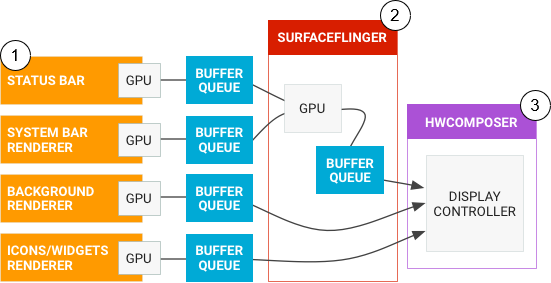
\includegraphics[width=13cm]{kththesis/Figures/android_graphics_pipeline.png}
    \caption[Graphic data flow through Android]{Graphic data flow through Android \footnotemark}
    \label{fig:android_data}
\end{figure}

\footnotetext{Source: \url{https://source.android.com/devices/graphics}}

Everything displayed on the screen has to go through SurfaceFlinger and the Hardware Composer.
\todo[inline, color=cyan!20]{Probably more clear now}
All these components synchronize with each other thanks to the VSYNC signal \cite{vsync}. When VSYNC signal is fired, all three components wake up at the same time: the Hardware Composer displays frame N, SurfaceFlinger takes a look inside the BufferQueue and composes frame N+1 if a new buffer is available, and the App Renderers generate frame N+2. The VSYNC signal depends on the device refresh rate, usually set at 60Hz though some new devices also support 90 or 120Hz \cite{refresh_rate}.

\paragraph{}
Application rendering itself is divided into 7 different stages \cite{app_rendering}:
\begin{enumerate}
    \item Input handling: executes input events callbacks
    \item Animation: executes animators callbacks
    \item Measurement and Layout: computes the size and position of all items
    \item Draw: generates the frame's drawing commands in the form of a display list
    \item Sync and Upload: transfers objects from CPU memory to GPU memory
    \item Issue commands: sends the drawing commands to the GPU
    \item Process and Swap buffers: pushes the frame's graphical buffer into the BufferQueue shared with SurfaceFlinger
\end{enumerate}

The Application rendering of Android's framework is synchronous as each stage will happen one after another. Only Input handling and Animation may not always happen depending on inputs and callbacks.

\subsection{Chrome}
Before understanding Chrome's rendering pipeline, it is best to first understand its architecture. It is based on multiple processes running at the same time, with each its specific function \cite{chrome_architecture} (see figure \ref{fig:chrome_architecture}):

\begin{itemize}
    \item Browser: controls everything related to the browser such as address bar, network requests and file access.
    \item GPU: displays all the elements on the screen by calling the OS's graphics library.
    \item Renderer: runs the web application. Each tab has its own Renderer sandboxed process with limited rights to protect the user and avoid crashing the browser.
    \item Plugin: runs the plugins used by the web application.
\end{itemize}

\begin{figure}
    \centering
    \includegraphics[width=13cm]{kththesis/Figures/chrome_architecture.png}
    \caption[Chrome's multi-process architecture]{Chrome's multi-process architecture \footnotemark}
    \label{fig:chrome_architecture}
\end{figure}

\footnotetext{Source: \textit{Inside look at modern web browser (part 1)} \cite{chrome_architecture}}

Each process also has several threads running at the same time for optimization.
 
\paragraph{}
Chrome's rendering pipeline \cite{chrome_pixel} contains similar stages as Android's application rendering but with some differences: 
\begin{enumerate}
    \item Parsing: translates the HTML into a DOM Tree.
    \item Styling: applies CSS style to DOM elements.
    \item Layout: computes the geometry of DOM elements (size and position) and produces a layout tree.
    \item Compositing: decomposes the page into layers which can be independently painted and rastered.
    \item Pre-painting: builds the property tree to apply to each layer.
    \item Painting: records paint operations into a list of display items.
    \item Tiling: divides the layers into tiles making its raster less expensive if only a part of it is needed
    \item Raster: executes the paint operations and decodes images to produce a bitmap.
    \item Drawing: generates a Compositor Frame and sends it to the GPU process.
\end{enumerate}
Every Renderer and the Browser Process can compute frames according to the pipeline described above. The GPU processes then aggregates all Compositor Frames according to the surface they represent on the screen and sends calls to the OS's graphics library. For Android, that means pushing a buffer of graphic data to SurfaceFlinger.
\newline
As opposed to Android, the output of the different stages are reused whenever possible. The frame is divided so that a small change in the frame only triggers a small amount of work to render it. 
For example scrolling only changes the position of a layer. There is no need to go through Parsing, Styling and Layout again. Pre-painting, Painting, Tiling and Raster may also be skipped if the size of the frame computed previously was bigger than the display screen.  

\section{Problem Analysis}

Though some security issues need to be resolved \cite{Pride_Prejudice}, Progressive Web Apps have the potential to become a popular cross-platform solution for developing mobile applications. They do not add much complexity to a regular web app \cite{JohannsenFabian2018PWAa}, greatly reduce the cost of developing a mobile application for every platform, and have similar performance than mobile applications regarding launch time \cite{PWApossibleUnifer}\cite{Biorn-Hansen2} \cite{PWAapplicability}, energy consumption \cite{PWAapplicability}, user experience \cite{emulating_native_w_crossplatform}\cite{PWA_UX_comparison_study}, or even hardware access in some cases \cite{PWAbc_responsetime}. 
\paragraph{}

However, at the time of writing no study that examined the User Interface performance at run-time was found. The User Interface performance can be divided into two main factors : the responsiveness (i.e. how fast the app can respond to user input), and the animation performance, (i.e. how well the transitions between two states are made, for example the animations when navigating, clicking a button, scrolling, changing content) which we will refer to as smoothness. This project will focus on studying the smoothness performance of mobile and progressive web apps.

The smoothness of a video is usually evaluated using the FPS rate, or frames per second \cite{smooth_gui}. It is also one of the main metrics recommended by Android\footnote{https://developer.android.com/training/testing/performance} and Google\footnote{https://developers.google.com/web/tools/chrome-devtools/evaluate-performance} to analyze the run-time performance of an application.\newline
However, this metric is not always considered relevant. Biørn-Hansen et al. \cite{animation_performance} examined several metrics used to evaluate animation performance in mobile application. They concluded that FPS was not a really useful information, especially for animations that runs only shortly and leave the application idle the rest of the time. Lin et al.\cite{smooth_gui} preferred to 
analyze the smoothness performance with jank, i.e. the number of non-updated screens displayed. Wen \cite{smoothnessQoE} instead considered 6 different indexes related to the frame intervals instead of the frame time. 

As there is no real consensus on the metrics to be used to analyze smoothness performance,  the first part of this study will focus on finding a relevant and measurable metric to compare the smoothness of android applications and Progressive Web Apps.

\paragraph{}
This chapter provided the necessary background to conduct this research and additional motivation. The next chapter will focus on the method of comparison of PWAs and Mobile Applications and the tools used to do so.
    

\chapter{Methodology}

The aim of this study is to compare the smoothness performance of mobile applications and Progressive Web Applications. We will reach this goal by answering 3 questions : How can we compare the smoothness of Progressive Web Applications and Mobile Applications? Are Progressive Web Applications as smooth as Mobile Applications? How efficient are they, that is how many resources are used to render a smooth application? \newline
This chapter will present the methods used to define a smoothness metric and to measure the resources consumed by the applications as well as the experiments used to evaluate the smoothness performance of the applications.


\section{Smoothness metric}
\label{method:smoothness}
    
    The smoothness of an application according to Android and Chrome is closely related to the frames displayed by the application. If a frame takes too long to be rendered, the user might notice some stuttering or freezing, resulting in a poorer quality of the User Experience. 
        
    The main source of graphical information for mobile applications on Android is the service \textit{gfxinfo} available with the command line \textit{adb shell dumpsys}. This service outputs several statistics about the application's frames, such as total number of frames rendered, the percentage of janky frames\footnote{Frames that were dropped or delayed} or the different timestamps of the most recent frames. Those timestamps can help developers identify the most time-consuming stage of the rendering pipeline and thus improve the smoothness of their application.
    
    \paragraph{}
    Another method to follow the computation of a frame on Android is to use the tool Systrace. With the relevant options selected, a developer can visualize the different functions called to compute a frame in a timeline as a flamegraph (see \autoref{fig:android_systrace_zoom}). \newline
    By looking at Android source code\footnote{\url{https://github.com/aosp-mirror/platform_frameworks_base/blob/master/core/java/android/view/Choreographer.java}}, it is possible to link the timestamps gathered by \textit{dumpsys gfxinfo} to the events displayed by Systrace (see \autoref{fig:android_frame_timeline}). 
    
    \begin{figure}
        \centering
        \includegraphics[width=13cm]{kththesis/Figures/android_systrace_zoom.JPG}
        \caption{Android Systrace - Screenshot}
        \label{fig:android_systrace_zoom}
    \end{figure}
    
    \begin{figure}[!ht]
        \centering
        \includegraphics[width=13cm]{kththesis/Figures/Android_frame_timeline.png}
        \caption{Linking Systrace and frame's timestamps - Screenshot with timestamps added}
        \label{fig:android_frame_timeline}
    \end{figure}

    \paragraph{}
    \autoref{fig:android_frame_timeline} gives an overview of the path taken by a frame on Android. Every frame starts with a VSYNC signal (first vertical red line in \autoref{fig:android_frame_timeline}), which acts as was presented in \autoref{background:pipeline:android} as a wake-up call for all the components of Android Graphics. The UI thread handles input and animation before measuring and computing the layout of the graphical elements. It updates the frame and hands it to the Renderer thread which issues the drawing commands and pushes the graphic buffer to SurfaceFlinger. To sum up, for Android a frame starts at VSYNC signal and is completed when its graphic buffer is pushed to SurfaceFlinger.
    
    \paragraph{}
    On Chrome, the frames follow a different pipeline as can be seen on \autoref{fig:pwa_systrace_zoom}, and thus remain undetected by Android system. Other tools specific to Chrome exist to collect the frame's duration of a web application, such as Chrome DevTools performance panel and Telemetry. Nevertheless, the inspection of their source code revealed that they define a frame duration as the interval between two consecutive frames, making those tools useless for comparing PWA and mobile applications on Android.
    
    \begin{figure}
        \centering
        \includegraphics[width=13cm]{kththesis/Figures/pwa_systrace_zoom.JPG}
        \caption{PWA Systrace - Screenshot}
        \label{fig:pwa_systrace_zoom}
    \end{figure}
    
    \paragraph{}
    Comparing the smoothness of Native Android, Hybrid and Progressive Web Applications requires a detailed overview of a frame's rendering pipeline, both on Chrome and Android. The latter provides it with the frame's timestamps gathered by \textit{dumpsys gfxinfo}. No documentation or tool was found to provide a similar overview of a frame's pipeline on Chrome. However, Chrome Tracing tool can record and display many functions called by Chrome's processes.
    
    \paragraph{}
    Thus, a model of Chrome Graphics pipeline was built empirically with an iterative process. The events recorded by Chrome Tracing tool were processed by a script which tracked the start and end of the frames as predicted by the model. If any error was raised, a visualization of the events on Chrome Tracing tool and a revision of the code allowed either to fix a bug in the code or to change the model according to the events observed. \newline
    The model was first built with a single benchmark application with limited interactions. It was then confronted with 10 traces of 8 different PWAs from the Github repositories pwarocks\footnote{https://github.com/pwarocks/pwa.rocks} and awesome-pwa\footnote{https://github.com/hemanth/awesome-pwa} to include a wider range of interactions. This confrontation was done 3 times each, with new PWAs until no significant errors remained.
    
    Those errors were:
    \begin{itemize}
        \item \textbf{Edge effects}: the start and end of a recording can happen anywhere on a frame's timeline. Some events, which require previous events or child events according to the model can raise an error at the start or the end of recording. Those errors are kept to a minimum, but can still happen as the recording does not always start or end at the same time for all threads. They do not invalidate the model.
        \item \textbf{Additional surface}: as it will be explained in more details later, every frame rendered is actually composed of aggregated surfaces. Each iframe or video embedded in the PWA adds a surface and make it more difficult to follow the frames. As this project is limited to simple apps with no videos or third-party advertisement, those errors are ignored. They do not invalidate the model.
        \item \textbf{Bugs}: those errors are not explained by the model. However, they are varied and extremely scarce (1 error over 5 000 frames computed) and are not considered statistically significant.
    \end{itemize}

\section{Resources}

The smoothness performance of an application refers to how smooth it can be and how many resources it uses in the process. The main resources consumed when an application renders a frame is the Memory and the CPU. This section presents how those resources are evaluated in mobile and progressive web applications.     

\subsection{Memory}
The memory in mobile applications on Android can be inspected with the service \textit{meminfo} of \textit{adb shell dumpsys}. Filtering with the application package name, it takes a snapshot of its memory and outputs detailed information about the memory used such as the java and native heap, the memory used by the code or the total amount of memory used by the application. The most interesting information is the total amount of RAM used by the application

\paragraph{}
Without filtering, this command line outputs the total amount of RAM used for each process. The processes are also ordered by section: persistent, foreground, visible and cached among others. \newline
The foreground section is the most useful. When a mobile application is running, only its process appears on the foreground. In the case of PWA, 3 processes appear on the foreground:  chrome package, a sandboxed sub-process of chrome, and a privileged sub-process of chrome. Those represent respectively, the Browser process, the Renderer process and the GPU process. This means all three processes needs to be considered when measuring the memory used by a PWA. 

%\todo{Always talk about the three types of applications when you refer to them: "Native, Hybrid and PWa"}

\paragraph{}
\todo[inline, color=cyan!20]{Can I just erase since I don't look at graphic buffers? because it will just repeat the preceding paragraph}
Two aspects of memory will be measured to compare Native, Hybrid and Progressive Web Apps: the RAM and the memory used for graphics buffer queue. For Progressive Web Apps, those measures will be the result of the addition of the 3 processes on the foreground: the Browser, the Renderer and the GPU processes.
    
\subsection{CPU}

There are 2 command lines that can be used to measure CPU usage of mobile applications on Android: \textit{adb shell top} and \textit{adb shell dumpsys cpuinfo}. \textit{Top} is similar to the Linux command of the same name, but with limited options. On Android, it is not possible to change the display from percentage of total CPU available to percentage of CPU core. This makes it less accurate than \textit{dumpsys cpuinfo} which displays the percentage of CPU core. Thus, \textit{dumpsys cpuinfo} will be used to measure CPU usage of mobile applications. 

\paragraph{}
The same command line can be used for Progressive Web Apps by adding the CPU usage of the 3 main processes (Browser, Renderer, GPU). 
However, some CPU usage measured by dumpsys might not come from the application in itself but from some other tasks done by the browser, or other web applications running on the background. 
Thus, other ways to obtain the CPU usage of the application were looked into.
The CPU graph from Chrome Devtools performance panel and the cpuTime computed for each frame were considered inadequate as they compute the self-time of the recorded functions, and not their CPU usage. The CPU sampling events saved during a recording promised more accurate measures \cite{cpu_sampling}. This method for measuring CPU was evaluated against Android's method with a single-core emulated device and a Progressive Web App able to trigger different CPU workloads. \newline

\paragraph{}
Because of the results presented in \autoref{sec:result_cpu}, Android's method will be used to extract CPU usage. The experiments will be done in airplane mode to minimize the overhead of the browser. 




\section{Devices}
\label{method:emulators}

Since emulators can provide easy access to a large range of Android devices, their use was considered for the final experiments. the CPU, of which the usage is a key metrics used to evaluate the performance of the applications, is a hardware difficult to emulate \cite{cpu_emulator}. Thus, it is important to test the emulators against a physical device before using them in CPU-related experiments.

As was presented in the background, only a few Android emulators do not enhance the hardware capabilities of the emulated device. Only 3 were identified and tested : Android Emulator, Genymotion and Visual Studio Android Emulator. As was explained previously, the metrics used to compare the performance of the emulators were the CPU usage using \textit{dumpsys cpuinfo}, the total RAM used using \textit{dumpsys meminfo} and the percentage of janky frames using \textit{dumpsys gfxinfo}. The measures were taken while the devices ran the same application that changed a text every few milliseconds. No human interaction was necessary. \newline

\section{Benchmark application and protocol}

A total of 3 benchmark applications were developed for this project: a Native Android app, a Hybrid app using React Native and a PWA using ReactJS. The frameworks React Native and ReactJS were chosen for the Hybrid and PWA because of their popularity and their similarity. Their common library 'react' and common architecture logic reduce the performance difference that can be introduced by the use of different frameworks.

\paragraph{}
Because of the empirical model and the smoothness metric found in \autoref{results:chrome_model} and \autoref{results:metric} all the applications contain the same features: a Clicking screen where the user can change the content by clicking on the screen, a Scrolling screen where the user can scroll the page to see all the content available and a Home screen where the user can navigate to the Clicking or the Scrolling screen. The content can be changed from text to picture and vice-versa. The screenshots of the applications are available in figures \ref{fig:native_screens}, \ref{fig:hybrid_screens} and \ref{fig:pwa_screens}.

\begin{figure}
    \centering
    \subcaptionbox{Home}{\includegraphics[width=2.1cm]{kththesis/screenshots/native_home.png}}
    \hfill
    \subcaptionbox{Clicking - text}{\includegraphics[width=2.1cm]{kththesis/screenshots/native_clicking_text.png}}
    \hfill
    \subcaptionbox{Clicking - picture}{\includegraphics[width=2.1cm]{kththesis/screenshots/native_clicking_picture.png}}
    \hfill
    \subcaptionbox{Scrolling - text}{\includegraphics[width=2.1cm]{kththesis/screenshots/native_scrolling_text.png}}
    \hfill
    \subcaptionbox{Scrolling - picture}{\includegraphics[width=2.1cm]{kththesis/screenshots/native_scrolling_picture.png}}
    \caption{Native application}
    \label{fig:native_screens}
\end{figure}

\begin{figure}
    \centering
    \subcaptionbox{Home}{\includegraphics[width=2.1cm]{kththesis/screenshots/hybrid_home.png}}
    \hfill
    \subcaptionbox{Clicking - text}{\includegraphics[width=2.1cm]{kththesis/screenshots/hybrid_clicking_text.png}}
    \hfill
    \subcaptionbox{Clicking - picture}{\includegraphics[width=2.1cm]{kththesis/screenshots/hybrid_clicking_picture.png}}
    \hfill
    \subcaptionbox{Scrolling - text}{\includegraphics[width=2.1cm]{kththesis/screenshots/hybrid_scrolling_text.png}}
    \hfill
    \subcaptionbox{Scrolling - picture}{\includegraphics[width=2.1cm]{kththesis/screenshots/hybrid_scrolling_picture.png}}
    \caption{Hybrid application}
    \label{fig:hybrid_screens}
\end{figure}

\begin{figure}
    \centering
    \subcaptionbox{Home}{\includegraphics[width=2.1cm]{kththesis/screenshots/pwa_home.png}}
    \hfill
    \subcaptionbox{Clicking - text}{\includegraphics[width=2.1cm]{kththesis/screenshots/pwa_clicking_text.png}}
    \hfill
    \subcaptionbox{Clicking - picture}{\includegraphics[width=2.1cm]{kththesis/screenshots/pwa_clicking_picture.png}}
    \hfill
    \subcaptionbox{Scrolling - text}{\includegraphics[width=2.1cm]{kththesis/screenshots/pwa_scrolling_text.png}}
    \hfill
    \subcaptionbox{Scrolling - picture}{\includegraphics[width=2.1cm]{kththesis/screenshots/pwa_scrolling_picture.png}}
    \caption{Progressive Web App}
    \label{fig:pwa_screens}
\end{figure}

\paragraph{}
The experiments will test 4 different scenarios : changing a text, changing a picture, scrolling a text and scrolling pictures. The frame duration, the CPU and memory usage will be measured separately for PWAs in order to minimize the overhead caused by the profiling tools. \newline
Because of the tool's limitation, clicking will be recorded for 25s and scrolling for 3s before extracting a memory snapshot and the CPU usage of the recording time. All the metrics will be measured at the same time for the native and hybrid applications. For the Progressive Web Apps, the frames and the resources used will be measured in separate experiments in order to avoid the overhead that the trace recording might cause.

\section{Technical contribution}

The scripts that were implemented to conduct this study are available on Git repository and are presented here. One of the main technical contribution of this study is the script modeling the rendering pipeline of Chrome. It analyzes the events recorded by Chrome Tracing tool and follows the computed frames from the moment they are requested to the moment they are pushed to SurfaceFlinger. The complete model of the script implemented is available in \autoref{annex:chrome_model}, with all the events tracked and the position of the timestamps on the pipeline.
\paragraph{}
Another contribution resides in the use of the experimental domain Tracing of the Chrome Devtools Protocol. It enables the automation of Trace recording and showed really useful in the automation of the experiments. The experimental methods \textit{Input.synthesizeTapGesture} and \textit{Input.synthesizeScrollGesture} were also used with great success.
\paragraph{}
Ultimately, all experiments were automated in order to remove the human interaction variable from the results and make them reproducible. This was done using monkeyrunner for experiments with \textit{dumpsys} and Chrome Devtools Protocol for experiments with trace recording.

\paragraph{}
This chapter presented the method used to find a relevant metric to compare the smoothness performant of Mobile and Progressive Web Apps and the benchmark applications developed to answer the second research question. The results of the various experiments and the empirical model of Chrome will be follow in the next part.

\chapter{Results}

This chapter will present the results of the experiments described in the previous part. It includes the empirical model of Chrome's rendering pipeline, the smoothness metric derived from it and the results of the experiments regarding emulators, CPU usage and lastly, the smoothness performance of Mobile Applications and Progressive Web Apps.

\section{Emulators}

As was explained in \autoref{method:emulators}, the CPU usage is difficult to simulate and thus Android emulators may not be as accurate as physical devices. This metric, along with the memory usage and the rate of janky frames were measured on different emulators and the corresponding physical device. All devices ran the same native application that required no human interaction. The results presented in \autoref{tab:memulators_test} are the average of 110 measurements.

\begin{table}[!ht]

    \resizebox{\textwidth}{!}{
    %\centering
    \begin{tabular}{|m{2,5cm}|m{2cm}|m{2cm}|m{2cm}||m{2cm}|m{2,5cm}|}
        \hline
         & \multicolumn{3}{c||}{Samsung S6 (API 7.0)} & \multicolumn{2}{|c|}{Samsung S5 (API 5.0)}  \\
         \hline
         Metrics & Physical device & Genymotion & Android Emulator & Physical device & Visual Studio Emulator \\
         \hline
         CPU Usage (\%) & 72 & 29 & 18 & 48 & 16 \\
         \hline
         RAM (KB) & 72 080 & 24 243 & 17 499 & 56 813 & 16 992 \\
         \hline
         Janky frames (\%) & 13 & 46 & 6 & 3 & 98 \\
         \hline
    \end{tabular}
    }
    \caption{Emulators Tests}
    \label{tab:memulators_test}
\end{table}

\paragraph{}
The results between the physical devices and the emulators are too different to be used in future experiments. Thus, only the available Android smartphones will be used for this project: Samsung S6 (Android version 7.0), Samsung S5 (Android version 5.0) and Samsung Galaxy S (Android version 4.2)


\section{CPU usage in Progressive Web Apps}
\label{results:cpu}
Since the CPU usage of PWA measured by \textit{dumpsys cpuinfo} may contain browser tasks that have nothing to do with the PWA, other measurement methods provided by Chrome were considered. One of them is the CPU sampling method executed by Chrome DevTools performance panel during a recording. 
Different CPU workloads were simulated with a function called at different time intervals. The CPU usage for each workload is the average of 100 measurements. The results are presented in \autoref{fig:cpu_usage}.

\begin{figure}
    \centering
    \includegraphics[width=13cm]{kththesis/Figures/cpu_graph.JPG}
    \caption[Measurements of CPU Usage of PWA]{Measured CPU usage (\%) over CPU workload represented by time laps between function calls}
    \label{fig:cpu_usage}
\end{figure}

As was expected, the CPU usage of the Renderer process (where the application lives) and the GPU Process decrease with the frequency of the function call. The CPU usage of the Browser process, though small, also decreases. This is surprising as the function call used to emulate CPU workloads did not involve the Browser in anyway. This indicates that the Browser process is necessary to run the PWA and not only at launch-time, to make network requests or to display an graphic element belonging to the Browser.

\paragraph{}
The curve of the CPU usage measured by Chrome's CPU sampling is closest to the curve of the CPU usage measured by \textit{dumpsys cpuinfo}. This indicates that it is a good estimation of the CPU usage of Chrome. However, it surpasses the measurements taken by \textit{dumpsys cpuinfo}. As the latter takes its measurements from the system files which count every tick of the CPU, it gives an accurate measurement of the CPU usage of Chrome. The Progressive Web App which is run by Chrome cannot exceeds its CPU usage. Thus, the CPU sampling method of Chrome is less accurate than \textit{dumpsys cpuinfo} to measure the CPU usage of a PWA. Later measurements of CPU will all be given by \textit{dumpsys cpuinfo}.

\section{Smoothness Metric}

To compare the smoothness performance of mobile and progressive web applications, a good understanding of their rendering pipeline is necessary. As no known document provides this understanding for Chrome, a model of Chrome's rendering pipeline was built empirically. This section presents the resulting model and the smoothness metric deducted from it. 

\subsection{Model of Chrome's Rendering pipeline}
\label{results:chrome_model}

Following the methodology proposed in \autoref{method:smoothness}, we formulate and describe the following model as the one used by Chrome to render contents in Android devices.

\paragraph{}
A frame in Chrome is an aggregation of several surfaces computed by different threads (See \autoref{fig:surface_diagram}). The App surface is computed by the Compositor thread and represents everything displayed by the application. The Browser surface computed by CrBrowserMain (referred to as Browser thread) represents everything displayed by the browser itself, for example the scrolling bar, the refreshing animation or the address bar in regular web applications. There can be more than two surfaces aggregated in a frame, for example if there is a video inside the web application or embedded ads.

\begin{figure}[h]
    \centering
    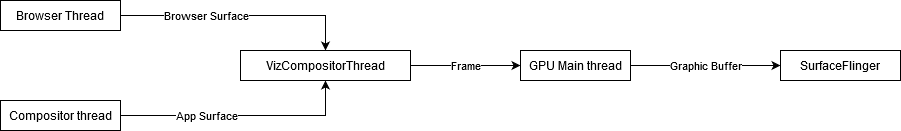
\includegraphics[width=13cm]{kththesis/Figures/surface_diagram.png}
    \caption{Surface Diagram}
    \label{fig:surface_diagram}
\end{figure}

\begin{figure}[h]
    \centering
    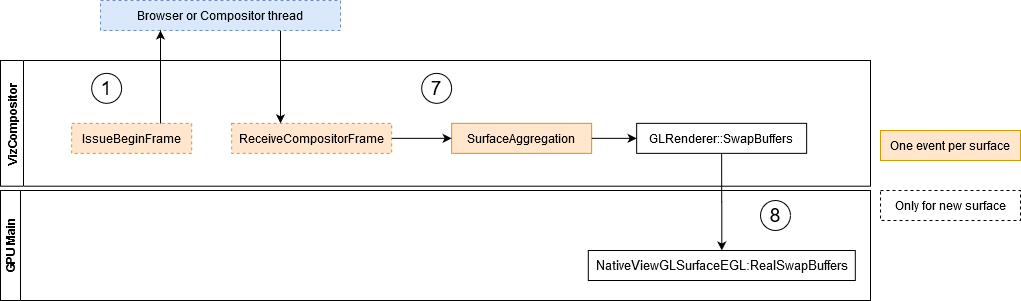
\includegraphics[width=\linewidth]{kththesis/Figures/Surface_aggregation.png}
    \caption{Surface aggregation}
    \label{fig:surface_aggregation}
\end{figure}

\paragraph{}
The VizCompositor thread manages all those surfaces (see \autoref{fig:surface_aggregation}). When a new frame is needed in reaction to user input or because of animations, it asks the Browser and/or the Compositor thread for a new surface and waits for them. Once it received all the new surfaces, it aggregates them into a single frame that it sends to the GPU thread. The latter is in charge of pushing the graphic buffer of the frame to SurfaceFlinger. 

\paragraph{}

\begin{figure}
    \centering
    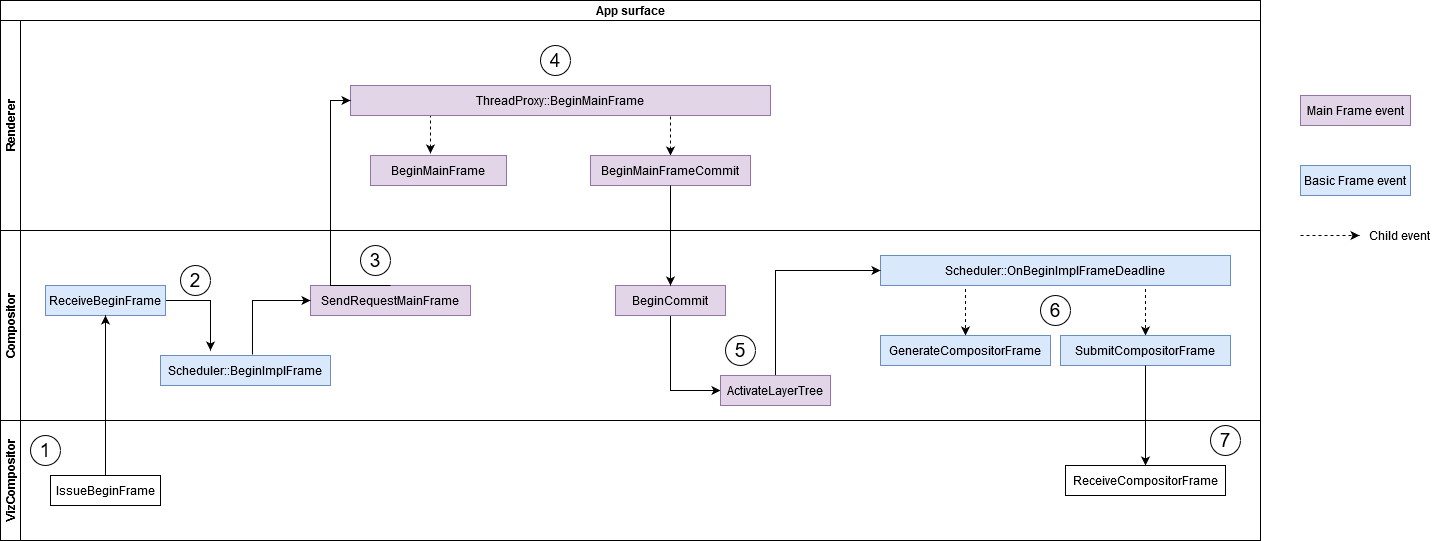
\includegraphics[width=\linewidth]{kththesis/Figures/App_surface.png}
    \caption{Model of an App surface}
    \label{fig:app_surface}
\end{figure}

The App surface can be computed in two different ways: a fast path, and a complete path. When there is only little changes to be made between two consecutive frames, the Compositor re-uses the baseline of the previous frame and only changes it slightly. This baseline is what we call a Main frame.
The \autoref{fig:app_surface} represents the main events involved in the computation of a new App surface. To summarize, a frame timeline with a new App surface is as follows:
\begin{enumerate}[ref={Step}\xspace\arabic*]
    \item \label{timeline:step1} The VizCompositor thread asks for a new frame to the Compositor thread.
    \item \label{timeline:step2} The Compositor thread agrees to compute a new frame and schedules it.
    \item \label{timeline:step3}The Compositor might also ask a new Main frame to the Renderer thread.
    \item \label{timeline:step4}If so, it compiles it. Regarding to the pipeline stages presented in the background, it computes the Styling, Layout, Compositing, Pre-Painting and Painting. When the Renderer thread is finished compiling the main frame, it commits it to the Compositor.
    \item \label{timeline:step5}When the Compositor receives a new Main frame, it computes Tiling and Raster if necessary with the help of other threads. The Main frame can then be activated: it replaces the old main frame in the memory of the Compositor thread and can be used as a baseline for future frames.
    \item \label{timeline:step6} Once the deadline scheduled in \ref{timeline:step2} is up, the frame is drawn. This step is the last stage of pipeline presented in the background: Drawing. The Compositor generates a CompositorFrame (or surface) and sends it to the VizCompositor.
    \item \label{timeline:step7}The VizCompositor waits for all necessary surfaces, aggregates them into a single frame and sends it to the GPU thread.
    \item \label{timeline:step8}Finally, the GPU thread receives the frame and pushes the graphic buffer to SurfaceFlinger
\end{enumerate}

The fast path can be used when only small changes occur between two consecutive frames and no stages present in \ref{timeline:step4} are necessary. It is the case for example when scrolling or for some CSS animations. The fast path can also be used when \ref{timeline:step4} takes too long to compute. The Compositor renders a new frame with fewer changes than planned, and the Main Frame being computed will be rendered with the next frame.
\paragraph{}
A frame timeline with a new Browser surface is similar to a new App surface. The main difference is that a Browser surface always follows a complete track and it is computed entirely on the Browser thread.

\subsection{Choice of smoothness metric}
\label{results:metric}

A frame timeline is very different on Chrome and Android. 
On one hand, Android's pipeline is synchronous and always follows the same path. The OS sends VSync signals depending on the device refresh rate, asking everything on the foreground to render a frame. In response, the UI thread calls Choreographer\#doFrame which handles callbacks for input and animation before doing some sizing and layout. The Choreographer then hands what it computed to the RenderThread which issues the draw commands and swap the buffers for SurfaceFlinger.

\paragraph{}
 on the other hand, Chrome's pipeline is flexible and depends on a lot of parameters. The VizCompositor also calls the Choreographer regularly after VSYNC signals but stop the process at animation callbacks. On Chrome's pipeline, the VizCompositor is also the one to start the frame. One animation callback of the Choreographer might trigger the start of the frame on VizCompositorThread, but no documentation is available to confirm this hypothesis and to give the time span between VSYNC signal and the start of the frame in Chrome. \newline
Thus, it is meaningless to compare Chrome's frames with Android's from VSYNC signal.

\paragraph{}
Another method is to compare the time it takes to swap buffers from the moment it decides to compute a new frame. That means from the start of the Choreographer for Android and the 'IssueBeginFrame' event for Chrome according to the empirical model. However, 'IssueBeginFrame' which is considered the start of the frame on Chrome might be triggered by other events that were not detected. Moreover, while Android starts computing the frame immediately, Chrome only schedules the computation of the frame. Thus, it can take into account not only events that happened before scheduling the frame but also before computing it.  
Therefore, this measure would be too inaccurate on Chrome. \newline


The last possible comparison is the amount of time Chrome and Android spent on computing the frame before swapping buffers. For Android, it starts with 'Traversal', and can be accessed with the \textit{PerformTraversalStart} timestamp. For Chrome, it depends on the type of frame pushed to SurfaceFlinger. We formulate the following 4 main issues:
\begin{enumerate}
    \item \textbf{When do Chrome starts computing a Main Frame?} \newline
    As the first stages of Chrome's pipeline happens in \ref{timeline:step6}, when the Renderer thread comes into play, the beginning of this step will be considered the start of the computation of a Main Frame.
    \item \textbf{When do Chrome starts computing a Basic Frame that re-uses a Main Frame?} \newline
    The only stage of Chrome's pipeline computed in a Basic Frame is Drawing, which begins at \ref{timeline:step6}. Thus, it will be considered the start of the computation of a Basic Frame.
     %\todo{add cross reference. Done in this case, use the same if you need to add more from here on}
    \item \textbf{Do frames which only changes the Browser surface count as frames to compare to mobile applications on Android?} \newline
    The Browser surface represents on PWA what is usually also handled by the application on Android (scrollbar, refresh animation). Thus, those frames will also be compared to Android frames. 
    \item \textbf{When both the App surface and the Browser surface changes, what to consider the start of the frame?} \newline
    Since they are pushed to SurfaceFlinger as a single frame, the start of the frame will be the start of the Browser or the App surface depending on which happens the earliest. 
\end{enumerate}

\paragraph{}
Therefore, Android and Chrome frames will be compared with their duration, that is from the time Android and Chrome start actively computing the frame until the buffers are swapped. 

\section{Smoothness Performance}

To compare the smoothness performance of Native, Hybrid and Progressive Web Applications, the average frame duration as defined in \autoref{results:metric}, the CPU and the Memory usage were measured in 4 different scenarios: 
\begin{enumerate} [ref={Scenario}\xspace\arabic*]
    \item \label{scenario:text:changing} Changing a text (\autoref{tab:text:changing})
    \begin{table}[]
        \centering
        \begin{tabular}{|c|c|c|c|}
            \hline
             & Native & Hybrid & PWA \\
             \hline
            \textbf{Samsung S6} &   &   &   \\
            Frame (ms) & 16,50 & 13,46 & 27,62 \\
            CPU (\%core) & 7,97 & 59,59 & 28,28 \\
            Memory (MB) & 68 & 196 & 257 \\
            \hline   
            \textbf{Samsung S5} &   &   &   \\
            Frame (ms) & 14,38 & 10,43 & 21,99 \\
            CPU (\%core) & 3,63 & 44,89 & 15,09 \\
            Memory (MB) & 47 & 169 & 148 \\
            \hline
            \textbf{Huawei P9 Lite} &   &   &   \\
            Frame (ms) & 10,47 & 6,50 & 22,47 \\
            CPU (\%core) & 4,03 & 31,44 & 22,35 \\
            Memory (MB) & 50 & 243 & 276 \\
            \hline
        \end{tabular}
        \caption{Changing a text}
        \label{tab:text:changing}
    \end{table}

    \item \label{scenario:text:scrolling} Scrolling a text (\autoref{tab:text:scrolling})
    \begin{table}[]
        \centering
        \begin{tabular}{|c|c|c|c|}
            \hline
             & Native & Hybrid & PWA \\
             \hline
            \textbf{Samsung S6} &   &   &   \\
            Frame (ms) & 17,32 & 18,40 & 24,71 \\
            CPU (\%core) & 40,13 & 90,03 & 105,63 \\
            Memory (MB) & 77 & 377 & 179 \\
            \hline   
            \textbf{Samsung S5} &   &   &   \\
            Frame (ms) & 3,85 & 5,19 & 21,96 \\
            CPU (\%core) & 28,57 & 59,42 & 66,86 \\
            Memory (MB) & 49 & 341 & 243 \\
            \hline
            \textbf{Huawei P9 Lite} &   &   &   \\
            Frame (ms) & 4,46 & 6,81 & 22,09 \\
            CPU (\%core) & 20,18 & 73,55 & 105,33 \\
            Memory (MB) & 55 & 406 & 149 \\
            \hline
        \end{tabular}
        \caption{Scrolling a text}
        \label{tab:text:scrolling}
    \end{table}
    \item \label{scenario:picture:changing} Changing a picture (\autoref{tab:picture:changing})
    \begin{table}[]
        \centering
        \begin{tabular}{|c|c|c|c|}
            \hline
             & Native & Hybrid & PWA \\
             \hline
            \textbf{Samsung S6} &   &   &   \\
            Frame (ms) & 9,66 & 9,48 & 17,86 \\
            CPU (\%core) & 9,09 & 57,82 & 25,66 \\
            Memory (MB) & 87 & 300 & 349 \\
            \hline   
            \textbf{Samsung S5} &   &   &   \\
            Frame (ms) & 17,04 & 7,83 & 15,67 \\
            CPU (\%core) & 8,41 & 44,36 & 11,56 \\
            Memory (MB) & 56 & 265 & 193 \\
            \hline
            \textbf{Huawei P9 Lite} &   &   &   \\
            Frame (ms) & 10,07 & 4,83 & 13,07 \\
            CPU (\%core) & 8,99 & 32,09 & 19,36 \\
            Memory (MB) & 56 & 317 & 316 \\
            \hline
        \end{tabular}
        \caption{Changing a picture}
        \label{tab:picture:changing}
    \end{table}
    \item \label{scenario:picture:scrolling} Scrolling pictures (\autoref{tab:picture:Scrolling})
    \begin{table}[]
        \centering
        \begin{tabular}{|c|c|c|c|}
            \hline
             & Native & Hybrid & PWA \\
             \hline
            \textbf{Samsung S6} &   &   &   \\
            Frame (ms) & 13,36 & 17,44 & 24,31 \\
            CPU (\%core) & 34 & 106,68 & 102,65 \\
            Memory (MB) & 106 & 578 & 182 \\
            \hline   
            \textbf{Samsung S5} &   &   &   \\
            Frame (ms) & 3,38 & 4,62 & 21,31 \\
            CPU (\%core) & 37,21 & 60,35 & 66,35 \\
            Memory (MB) & 104 & 283 & 243 \\
            \hline
            \textbf{Huawei P9 Lite} &   &   &   \\
            Frame (ms) & 4,57 & 7,63 & 22,31 \\
            CPU (\%core) & 51,13 & 116,37 & 119,17 \\
            Memory (MB) & 97 & 614 & 154 \\
            \hline
        \end{tabular}
        \caption{Scrolling pictures}
        \label{tab:picture:Scrolling}
    \end{table}
\end{enumerate}

First, we will mention some issues that were raised during and after the experiments. Then, we will present several observations that can be made from result. \newline

\subsection{Experiment notes}
The results presented here are the average of 100 measures. However, some small issues were raised during and after the experiments.\newline
Firstly, the scrolling experiments were not as consistent between frameworks and devices as changing content was. The same drag event did not trigger the same scrolling speed, and the length of the scrolling page was different. The tools used to simulate drag events also behaved  differently. Thus, the drag events were adapted to the device and framework so that the view scrolled all the way down and a little up during the experiments. \newline
Lastly, the clocks of different threads in Chrome were sometimes found to be slightly out of sync. Thus, some events were detected before their triggering events on another thread. However, those incidents concerned events not counted in the frame duration. They were scarce and the delay was of small magnitude. Thus, it was concluded that they did not impact the results presented here.

\subsection{Takeaways}
\label{results:performance}
The first observation is the difference of frame computation time of the same application between devices. In both Scrolling scenarios (\autoref{tab:picture:Scrolling} \autoref{tab:text:scrolling}), the Native and Hybrid applications takes 3 or 4 times more time to compute a frame on Samsung S6 than on Samsung S5 and Huawei. The difference is less significant on Changing Scenarios though a two-times magnitude difference can still be observed. PWAs also offer a more consistent smoothness over devices.
\paragraph{}
The second observation concerns only the Progressive Web App. With the metric defined in \autoref{results:metric}, it was expected that scrolling would result in smaller frame computation times for PWA. This is true when displaying text though the difference is small, but not at all when displaying pictures. \todo[color=cyan!20]{I have no idea why}

\paragraph{}
The third observation concerns the resources used by the applications. The Native application consumes significantly less CPU and Memory than the Hybrid and Progressive Web Application in every scenario. On the one hand, the Native application consumes only around 50 MB of RAM, 100MB at most when scrolling pictures. On the other hand, the PWA and Hybrid app consumes at least 150 MB of RAM and even up to 600 MB for the Hybrid application.  \newline
The difference of CPU consumption is not as big, but still significant with a 2 times magnitude difference between the Native and the Hybrid and PWA, sometimes more. The Hybrid application consumes slightly less CPU than the PWA during scrolling, while the PWA consumes less CPU than the Hybrid app when changing content. 

\paragraph{}
The last observation is a comparison of the Native and Hybrid applications. The performance of the Hybrid application is better when changing content while the Native application is better when scrolling. However, the Hybrid application only follows it by 2 or 3ms during a scroll, while the Native application can lag behind the Hybrid app by up to 10 ms. 

\paragraph{}
To summarize the results presented in this chapter, it was found that the CPU usage measured by Chrome tools is not as accurate as Android tools and that Android emulators are not precise enough to use them in CPU experiments. A smoothness metric able to compare Mobile applications and Progressive Web app was defined and used to compare a Hybrid, a Native and a Progressive Web Application. The next chapter will discuss those results.


\chapter{Discussion}

The last chapter presented the results of several experiments regarding Android emulators, measurements of CPU usage and smoothness performance. This chapter will discuss those results and their limitations.

\section{Limitations}
\todo[inline]{Move limitation as the last section of the chapter}
One of the main limitation of the results presented previously lies in the number of devices used for the experiments. As was observed in \autoref{results:performance}, the performance of the applications can differ greatly between devices. More experiments on other devices need to be conducted to validate the conclusion reached from the current results. \newline
A second limitation is the measurements of the resources used the Progressive Web app. As was mentioned in \autoref{results:cpu}, those measurements are less accurate than for the mobile applications because the browser may perform other tasks unrelated to the PWA. Those tasks were minimized during the experiments: the airplane mode was activated, the WiFi deactivated and no other web applications were present in the background. \newline
Another limitation comes from the limited cross-platform and Web framework used. The results presented here only applies to React Native and React as every framework has its own strength and weaknesses. 
The last limitation comes from the OS and browser studied during this project. Only Android and Chrome browser was studied even though other browsers and OS are used regularly by numerous people. Those other browsers and OS, especially Safari on iOS need to be studied before reaching a conclusion on the performance of Progressive Web Application compared to mobile applications.

\section{Smoothness metric}
The smoothness metric used to compare Mobile and Progressive Web Applications was defined using an empirical model of Chrome's rendering pipeline. Though this model is not usable for every web applications, it is consistent with the events observed in simple web applications and allowed a comparison of the frames computed by Chrome and by Android framework. Since the start of a frame is not triggered by the same events on Chrome and Android, the frame duration is defined as the time it takes to compute a frame and push it to SurfaceFlinger. However, this metric was identified only for applications running with Chrome browser on Android. Other smoothness metrics might be used with other browsers and other OS. 

\section{Smoothness}
The smoothness performance of native, hybrid and progressive web applications was evaluated in 4 different scenarios as they triggered different stages of Chrome's rendering pipeline: changing a text, scrolling a text, changing pictures and scrolling pictures. In almost every scenario, the smoothness of the Progressive Web App was found to be lagging behind those of native and hybrid applications, often by a 2-time magnitude.\newline
Contrary to what was expected, the frame computation time of Progressive Web Apps when changing a picture was a lot better than when scrolling pictures. As this is not observed when the content is text, this might be due to a better usage of the GPU, though this is only a hypothesis. \newline
The Native and Hybrid application have similar results. The Hybrid app is faster at computing frames when changing the content displayed than the Native application, and slower when scrolling the view. As the difference is only of 2 or 3 ms during a scroll, and can attain 10 ms when changing content, the Hybrid application can be considered to be smoother than the Native application.


\section{Resource consumption}
The resources measured during the experiments were the CPU and Memory usage. The Native application was found to consume a lot less resources than the Hybrid and Progressive Web Applications. This will more likely impact the battery consumption, and corresponds to the result found by Ciman and Gaggi \cite{ciman2017empirical} who compared the energy consumption of Native and Cross-platform applications. They concluded that cross-platform applications consume more energy than native applications, especially when updating the User Interface. However, it does not concur the results found by Tjarco \cite{PWAapplicability} who compared the energy consumption of a Progressive Web App and Native applications and found that PWA consume less energy. Nevertheless, the applications used for his experiments also accessed the network regularly, impacting the results. Moreover, though a high CPU and Memory usage does consume more energy, it is not an accurate indicator of energy consumption.

The results achieved during this work were discussed as well as their limitations. The next chapter will conclude this work. 


\chapter{Conclusion}

This chapter concludes this study of Progressive Web Applications. First, the research questions will be answered with the work done during this study. Then, suggestions of future work related to Progressive Web Apps will be presented.

\section{Contributions}

The main research question revolves around the smoothness performance of Progressive Web Applications compared to Mobile Applications on Android. The smoothness performance refers in this work to how well frames are computed, and the efficient use of resources to do so. 
\paragraph{}
First, a model of Chrome's rendering pipeline was built empirically. This model allowed us to define a smoothness metric able to compare the frame duration of Mobile Applications on Android and Progressive Web Apps on Chrome. Since, the event triggering a new frame on Chrome is difficult to identify, and new events can impact the frame until late on Chrome's rendering pipeline, this metric was defined as the computation time of the frame before it is handled by the display manager of Android. 
\paragraph{}
This metric allowed us to compare the frame computation time of Mobile Applications and Progressive Web Apps with different user interactions and different type of content displayed. In all scenarios, the Progressive Web Application was a lot slower to compute a new frame than the Native and Hybrid Applications. Thus, we can conclude that Progressive Web Apps are not as smooth as Mobile Applications on Android.
\paragraph{}
The resources used, namely the CPU and the Memory were also measured to compare the efficiency of the applications when computing new frames. In all scenarios, the Native application was more efficient than the Hybrid and Progressive Web Application, both in terms of CPU and Memory. However, the efficiency of the Hybrid and the Progressive Web Application was similar. From this, we can infer that progressive Web Applications does not consume more resources than Hybrid applications, but Native Android Applications remain more efficient.

\paragraph{}
To summarize, we found that Progressive Web Applications are not as smooth as Mobile Applications on Android. Their resource consumption, though similar to Hybrid applications, is higher than Native Applications. With this, we can conclude the smoothness performance of Progressive Web Apps is not as smooth as Native and Hybrid Applications on Android. 

\section{Future work}
Several questions remains on the subject of Progressive Web Apps.One of them is the comparison of Progressive Web Application to Mobile applications on iOS. As the support of PWA on iOS is lagging behind Android, this comparison was often overlooked. \newline
The work conducted here on smoothness performance can also be extended to other browsers, other platforms and other cross-platform technologies. This work can also be extended to include the responsiveness of PWA and Mobile Applications, as it is an important aspect of the User Interface Performance. \newline
Other aspects of Progressive Web Apps can also be compared to Mobile applications, such as the development and maintenance efforts of the developers, and the engagement of the end users. \newline
The security aspect is also important to consider. Though Jiyeon et al. \cite{Pride_Prejudice} already opened the question, some questions remains, for instance the additional security flaws that threatens the integrity of Progressive Web Apps compared to regular web applications, and the possibility for end-users to install a malicious Progressive Web App as no organization inspect them.
Finally, as Progressive Web Applications can also be installed on desktop, they can also be compared to desktop applications. All the research conducted and suggested until now to compare them to Mobile Applications can be transferred to desktop applications. Though computers often have much almost unlimited resources than compared to smartphones, the resource's consumption still need to be studied as laptop do not always have an unlimited power source, and some have really limited CPU and memory. 


\listoftodos{Notes}

\listoffigures
\printbibliography[heading=bibintoc]

\appendix
    \chapter{Model of Chrome Rendering pipeline}
    \label{annex:chrome_model}
    
    \begin{center}
        \includegraphics[angle=90, height=17cm]{kththesis/Figures/Chrome_Graphics_v2.png}
    \end{center}


% Tailmatter inserts the back cover page (if enabled)
\tailmatter

\end{document}
